\documentclass[preprint,12pt]{elsarticle}

\usepackage{amssymb}
\usepackage{amsmath}
\usepackage{url}
\usepackage{tikz}
\usepackage{booktabs}
\usepackage{placeins}
\usetikzlibrary{arrows.meta,positioning,shapes.geometric}
\setlength{\floatsep}{8pt plus 2pt minus 2pt}
\setlength{\textfloatsep}{14pt plus 2pt minus 4pt}
\setlength{\intextsep}{8pt plus 2pt minus 2pt}
\journal{Knowledge-Based Systems}

\begin{document}

\begin{frontmatter}

\title{Decision-aligned eviction-value prediction for learning-augmented caching}

\author[label1]{Soroush Vahidi}
\ead{sv96@njit.edu}

\affiliation[label1]{organization={Ying Wu College of Computing, New Jersey Institute of Technology},
            city={Newark},
            state={NJ},
            country={USA}}

\begin{abstract}
Caching with predictive information remains challenging because predictions must be translated into eviction decisions, not merely assessed for accuracy. We study online paging from a candidate-level perspective: at each full-cache miss, the policy scores the items currently in cache and evicts the candidate with smallest predicted downstream harm under a finite-horizon replay target built from a fixed continuation rule. We instantiate this framework in unweighted paging and note, but do not empirically validate, an optional guarded fallback for locally unsafe learned decisions. Offline ablation shows that short-horizon nonlinear scorers learn the target most effectively. End-to-end online replay across seven trace families at capacities 32, 64, and 128 shows that the proposed policy does not improve on LRU, SIEVE, or FIFO-Reinsertion; the gap widens non-monotonically at the largest evaluated capacity. The results support finite-horizon eviction-value prediction as a learnable supervision-target design, while showing that the present instantiation is not yet a practically superior online replacement rule relative to strong lightweight baselines.
\end{abstract}

\begin{keyword}
learning-augmented caching \sep online paging \sep cache replacement \sep eviction-value prediction \sep caching baselines
\end{keyword}
\end{frontmatter}

\section{Introduction}
\label{sec:introduction}

\subsection{Problem Setting and Motivation}
\label{subsec:problem_motivation}

Caching is a fundamental systems mechanism for reducing latency, lowering backend load, and improving throughput in data-intensive services. In online caching, requests arrive sequentially, and when a miss occurs under full capacity, the policy must choose an eviction without access to future requests. Even in the classical paging setting, this local choice has important downstream consequences: a poor eviction can create avoidable future misses, whereas a better choice can preserve useful locality and reduce cumulative cost \cite{belady1966replacement_algorithms,fiat1991competitive_paging}.

Recent work on learning-augmented caching has shown that predictive information can improve online performance when it is informative and incorporated carefully into the replacement rule \cite{lykouris2021competitive_caching,antoniadis2020online_metric_untrusted,im2022parsimonious_lac}. At the same time, this literature also makes clear that predictive gains are highly regime dependent. Methods that perform well under one workload, cache size, or prediction model may degrade substantially when predictions are noisy, shifted, or weakly aligned with the actual replacement objective \cite{wei2020better_simpler_lac,chledowski2021robust_lac_experimental}. More broadly, this reflects a central theme in algorithms with predictions: predictive information is useful only when it improves the decision that the online algorithm must actually make \cite{mitzenmacher2022algorithms_predictions}.

This observation is especially important for practical cache control. At a full-cache miss, the relevant question is not merely whether a predictor should be trusted in the abstract, but which currently cached item is safest to remove. The replacement problem is therefore inherently a candidate-selection problem, and from this perspective the learning target matters. If learning is organized only around a coarse proxy, such as a trust signal or another indirect future hint, the resulting policy may remain weakly aligned with the eviction decision itself. By contrast, a candidate-level target asks a more direct question: what downstream harm is associated with evicting each available item under the current decision context?

This paper studies that candidate-centric view, modeling each full-cache miss as a structured comparison among the current eviction candidates rather than as a single global trust decision about a predictive hint. Section~\ref{subsec:objective_scope} states the resulting research objective and the three aims that follow from it.

\subsection{Research Objective and Scope}
\label{subsec:objective_scope}

Building on the candidate-centric premise introduced above, the objective of this study is to investigate a learning-augmented caching method whose supervision target is aligned with the eviction decision itself: the policy estimates the short-horizon downstream cost of evicting each item currently in cache and selects the candidate with the smallest predicted cost.

Within this perspective, the paper has three aims. First, it formulates eviction as a candidate-level value-prediction problem in the unweighted paging setting. Second, it develops an empirical framework for evaluating this decision rule against classical, predictive, and robust reference policies under a common replay protocol. Third, it studies whether lightweight fallback mechanisms can provide additional protection when learned decisions appear locally unsafe. Taken together, these aims position the work as a methodological and empirical study of decision-aligned cache control.

The scope of the paper is intentionally focused on standard online paging with fixed cache capacity and unit miss cost. We do not present a competitive-ratio guarantee for the learned policy, nor claim universal superiority over alternative learning-augmented formulations. The contribution is instead a decision-aligned supervision target, a candidate-scoring framework built on that target, and an empirical study of when this approach is useful.
\subsection{Main Contributions}
\label{subsec:main_contributions}

The main contributions of this paper are as follows.

\begin{enumerate}
    \item We formulate learning-augmented paging from a candidate-level decision perspective, in which each full-cache miss is treated as a structured comparison among the items currently stored in the cache. This reframes the use of predictive information around the quality of concrete eviction actions rather than around global trust in advice alone.

    \item We introduce an eviction-value prediction framework for online paging that uses short-horizon downstream replay to construct a decision-aligned supervision target for each eviction candidate. The resulting target is intended to model the local downstream harm of an eviction choice more directly than advice-only, action-imitation, or indirect proxy formulations.

    \item We provide a reproducible empirical framework for studying the proposed method against classical, predictive, and robust reference policies under common replay semantics, with explicit separation between offline scorer analysis and downstream online replay evaluation.

    \item We contribute an empirical and methodological perspective on decision-aligned cache replacement that highlights supervision-target design as a central issue in learning-augmented caching. In particular, the paper provides evidence that candidate-level finite-horizon eviction scoring is a plausible and practically grounded direction for integrating predictive context into online eviction decisions under imperfect predictive information.
\end{enumerate}

\subsection{Related Work}
\label{subsec:related_work}

The classical foundation of this problem lies in online paging and cache replacement, where eviction decisions must be made without access to future requests. Belady's offline rule provides the standard clairvoyant benchmark, while competitive paging established the canonical worst-case framework for reasoning about online replacement quality \cite{belady1966replacement_algorithms,fiat1991competitive_paging}. These works capture the central difficulty that remains in modern cache control: the quality of an eviction decision depends on future reuse, yet the decision itself must be made online.

Learning-augmented caching extends this setting by allowing the online algorithm to exploit predictive information. In the paging literature, this line has focused primarily on advice such as next-arrival predictions, predicted actions, and limited future-oriented queries, together with robustness guarantees when the advice is inaccurate \cite{lykouris2021competitive_caching,rohatgi2020near_optimal_caching,bansal2022learning_augmented_weighted_paging,im2022parsimonious_lac}. Closely related work on untrusted predictions and robust online algorithms studies how predictive decisions can be combined with safer fallback behavior or expert-style switching without sacrificing worst-case protection \cite{antoniadis2020online_metric_untrusted,wei2020better_simpler_lac,chledowski2021robust_lac_experimental,blum2000online_learning_mts}. Our work is aligned with this literature in its concern for robustness, but differs in emphasis: rather than centering the design on trust in a hint or on policy-level switching alone, we study a candidate-level supervision target tied directly to the eviction decision itself.

A second relevant line comes from learned cache-replacement systems that use future-derived supervision to guide eviction. PARROT learns to imitate Belady-style eviction behavior from trace-derived oracle decisions, while LRB and Raven use Belady-guided future-access prediction to drive learned replacement decisions \cite{liu2020parrot,song2020lrb,hu2022raven}. Mockingjay moves beyond binary Belady-style labels by learning finer-grained reuse-time estimates for eviction ordering \cite{shah2022mockingjay}. HALP is especially relevant because it uses candidate-level preference learning from future re-access outcomes rather than direct action imitation \cite{song2023halp}. These papers are close to the present work in that they move eviction learning beyond purely hand-designed heuristics. However, they are still organized around oracle imitation, next-arrival or reuse-distance prediction, or pairwise future preference signals, rather than explicit supervision on finite-horizon candidate-specific downstream harm. A faithful empirical reimplementation of HALP is outside the scope of the present revision; the comparison above is therefore analytical rather than empirical, and we treat this as an explicit scope limitation rather than an omitted result.

This distinction matters because, in many prior formulations, the learned quantity remains an intermediate proxy that must still be translated into an eviction action. Such proxies include oracle action labels, reuse-distance estimates, next-arrival forecasts, and pairwise candidate orderings \cite{liu2020parrot,shah2022mockingjay,hu2022raven,song2023halp}. By contrast, our formulation is motivated by the view that eviction is inherently a local action-selection problem, so the supervision target should approximate the downstream consequence of each available action as directly as possible. In this sense, the paper is conceptually closer to decision-focused learning and predict-then-optimize perspectives, even though those frameworks have not been developed explicitly for cache-replacement supervision in the paging literature \cite{elmachtoub2022smart_predict_optimize,wilder2019decision_focused_learning}.

The paper is also related to recent finite-horizon predictive approaches such as MUSTACHE, which uses multi-step-ahead page prediction to improve eviction decisions \cite{tolomei2022mustache}. That work is particularly relevant because it introduces an explicit forecasting horizon. Our method differs in what is supervised: rather than predicting future pages or arrival times and then deriving eviction decisions from those forecasts, we train directly on a finite-horizon eviction-cost target defined at the candidate level.

Our empirical comparison includes SIEVE and FIFO-Reinsertion as strong CLOCK-family lightweight baselines \cite{zhang2024sieve}. The repository associated with this paper supports heterogeneous public and production-style traces used as replay environments \cite{cho2011friendship_mobility,citibike_system_data,henning2006spec_cpu2006,wikimedia_pageviews,yang2020twitter_cache_clusters,waldspurger2015shards,cachemon_open_source_cache_dataset,cachelib_cachebench_fb_hw_eval}; these sources are not presented as new datasets.

\section{Main Method}
\label{sec:method}

\subsection{System Model and Preliminaries}
\label{subsec:system_model}

We study online caching in the standard unweighted paging setting. Let
\begin{equation}
\sigma = (r_1, r_2, \ldots, r_T)
\label{eq:req-seq}
\end{equation}
denote the request sequence, where each request $r_t \in \mathcal{P}$ refers to an item in a finite universe $\mathcal{P}$. The cache has capacity $k$, and its content immediately before serving request $r_t$ is denoted by $C_t \subseteq \mathcal{P}$ with $|C_t| \leq k$. If $r_t \in C_t$, the request is a hit; otherwise, it is a miss. When a miss occurs and the cache is full, that is, when $|C_t| = k$, the policy must evict one cached item before inserting $r_t$ \cite{belady1966replacement_algorithms,fiat1991competitive_paging}.

We focus on the unweighted setting because it isolates the eviction-choice problem while preserving clean comparison with classical, predictive, and robust baselines. Each miss incurs unit cost, so performance is measured primarily by total misses. If $m_t \in \{0,1\}$ denotes the miss indicator at time $t$, then the total cost over the sequence is
\begin{equation}
\mathrm{Cost}(\sigma) = \sum_{t=1}^{T} m_t.
\label{eq:total-cost}
\end{equation}

Learning-augmented caching enriches this online setting with predictive information that may help guide replacement decisions. Prior work has considered advice in the form of predicted next-arrival times, predicted cache states, and limited access to future-oriented signals \cite{lykouris2021competitive_caching,antoniadis2020online_metric_untrusted,im2022parsimonious_lac}. In this paper, such information is treated as auxiliary decision-time context rather than as an instruction that should be followed directly. The goal is therefore not only to assess whether a predictor is trustworthy, but to determine how available predictive context should influence the eviction decision at a full-cache miss.

Formally, when a miss occurs at time $t$ and $|C_t| = k$, the eviction candidates are the items currently stored in the cache:
\begin{equation}
\mathcal{V}_t = C_t.
\label{eq:candidate-set}
\end{equation}
The online action is to select some $q \in \mathcal{V}_t$ for eviction. Classical policies define this action through fixed rules such as recency or marking, whereas predictive policies often derive it from a forecast or advice signal \cite{fiat1991competitive_paging,lykouris2021competitive_caching}. Our perspective is different: we evaluate an eviction by its downstream effect on future misses.

To make this idea operational, we define a finite-horizon candidate loss. For a candidate $q \in \mathcal{V}_t$ and horizon $H \geq 1$, let
\begin{equation}
L_H(q,t) = \sum_{\tau=t+1}^{t+H} m_{\tau}^{(q,t)}
\label{eq:horizon-loss}
\end{equation}
denote the number of misses incurred over the next $H$ requests after forcibly evicting $q$ at time $t$ and replaying the subsequent cache evolution under a fixed continuation rule. Here, $m_{\tau}^{(q,t)} \in \{0,1\}$ is the miss indicator at time $\tau$ under that counterfactual trajectory. In the implementation studied here, the continuation rule is a lightweight LRU-style replay. This yields a deterministic and computationally tractable supervision target. It should be interpreted as a local proxy for the downstream harm of an eviction choice, not as an offline-optimal objective.

This candidate-level formulation is the central shift of the method. Instead of asking only whether a predictive signal should be trusted, we ask which currently cached item appears least costly to remove under the present state and context. The remainder of the method section builds on this formulation to define the learned scoring rule and then introduces practical fallback behavior for settings in which learned decisions appear unreliable.
\subsection{Eviction-Value Prediction Framework}
\label{subsec:eviction_value_framework}

The central idea of the proposed method is to replace coarse trust-oriented control with a direct estimate of \emph{eviction quality} at decision time. Consider a miss at time $t$ when the cache is full, so that the candidate set is $\mathcal{V}_t = C_t$. Instead of asking only whether a predictive signal should be followed, the method assigns each candidate $q \in \mathcal{V}_t$ a score that estimates the downstream harm of evicting that candidate under the current context. The selected victim is then the candidate with the smallest predicted loss.

Let $H \geq 1$ denote a finite replay horizon. For a candidate $q \in \mathcal{V}_t$, define its horizon-$H$ eviction loss by
\begin{equation}
L_H(q,t) = \sum_{\tau=t+1}^{t+H} m_{\tau}^{(q,t)},
\label{eq:eviction_loss}
\end{equation}
where $m_{\tau}^{(q,t)} \in \{0,1\}$ is the miss indicator at future step $\tau$ under a counterfactual trajectory in which $q$ is evicted at time $t$ and the subsequent cache evolution is replayed under a fixed continuation rule. In the current implementation, the default continuation rule is a lightweight LRU-style replay. This choice yields a deterministic and computationally tractable supervision signal and serves as a practical approximation rather than a claim of optimal continuation. Alternative continuation rules are treated as exploratory sensitivity directions rather than part of the main method.

The quantity in \eqref{eq:eviction_loss} is not an offline optimum. Rather, it is a local proxy for the downstream harm of an eviction choice. This is the key modeling shift of the framework. Prior learned caching methods often predict a proxy such as next arrival, reuse distance, an oracle-derived action, or a pairwise preference. Here the supervision target is tied more directly to the actual online decision: among the currently cached items, which one appears least costly to remove over a short lookahead window?

At each decision time, the framework constructs a feature vector for every candidate $q \in \mathcal{V}_t$,
\begin{equation}
x(q,t) \in \mathbb{R}^{d},
\label{eq:feature_vector}
\end{equation}
where the features summarize the current request, the cache state, and candidate-specific predictive context. In the current repository, these features are organized into a small number of interpretable groups, including request-side features, candidate-side recency and reuse features, predictor--LRU comparison features, cache-state summary features, disagreement features, and recent-activity features. When predictive metadata are available, they are incorporated through these feature groups rather than treated as hard instructions. Table~\ref{tab:evict-value-feature-groups} summarizes the feature families used by the scorer.

The learned scorer is a function
\begin{equation}
\widehat{L}_H(q,t) = f_{\theta}\!\left(x(q,t)\right),
\label{eq:predicted_loss}
\end{equation}
and the eviction decision becomes
\begin{equation}
q_t^{*} = \arg\min_{q \in \mathcal{V}_t} \widehat{L}_H(q,t).
\label{eq:eviction_rule}
\end{equation}

The replay target in \eqref{eq:eviction_loss} forms the basis for the optional guarded fallback mechanism described next.

\begin{table}[!htbp]
\centering
\caption{Decision-time feature groups used by the eviction-value scorer. The table summarizes the main feature families implemented in the current artifact pipeline; the full feature specification is repository-based and reproducibility-oriented.}
\label{tab:evict-value-feature-groups}
\small
\begin{tabular}{p{3.3cm} p{9.6cm}}
\toprule
Feature group & Role in decision-time scoring \\
\midrule
Request-side features & Encode properties of the current request and its immediate decision context. \\
Candidate-side reuse and recency features & Summarize candidate age, recent reuse behavior, and local history relevant to eviction risk. \\
Predictor--LRU comparison features & Capture how predictive context differs from recency-based signals for the same candidate. \\
Cache-state summary features & Describe the current cache composition and local competition among candidates. \\
Disagreement features & Indicate whether predictor-oriented and recency-oriented views point to different eviction choices. \\
Recent-activity features & Summarize short-window request activity and local workload dynamics near the decision point. \\
\bottomrule
\end{tabular}
\end{table}

\subsection{Guarded Fallback Mechanism}
\label{subsec:guarded_fallback_mechanism}

A learned eviction scorer can improve decision quality when its candidate rankings are well aligned with future reuse, but its behavior may deteriorate when the workload changes or when local predictive context becomes unreliable. We therefore describe a lightweight optional guard that can temporarily delegate to a conservative fallback when recent online behavior suggests locally unsafe learned decisions; we treat this guard as an implementation safeguard for future empirical study rather than as a demonstrated component of the present results (see Limitations).

The guard uses repeated \emph{very-early-return} evictions as its signal. Let $q_t^{*}$ denote the victim proposed by the learned scorer at time $t$. If the evicted item is requested again within a short window, the decision is treated as suspicious because it indicates that an item with immediate reuse value may have been removed.

Formally, let
\begin{equation}
E_t =
\begin{cases}
1, & \text{if the item evicted at time } t \text{ returns within } W \text{ subsequent requests},\\
0, & \text{otherwise},
\end{cases}
\label{eq:early_return_signal}
\end{equation}
where $W$ is a small early-return window. The mechanism aggregates these suspicious events over a sliding interval of length $T$. Writing the recent suspicious count as
\begin{equation}
S_t = \sum_{\tau=\max(1,t-T+1)}^{t} E_{\tau},
\label{eq:suspicious_count}
\end{equation}
the trigger condition is
\begin{equation}
S_t \geq M,
\label{eq:guard_trigger}
\end{equation}
where $M$ is the threshold required to enter fallback mode.

Once triggered, the controller temporarily delegates the eviction choice to a conservative fallback policy for a bounded duration $D$. In the current implementation, the fallback is configurable and may be instantiated by a simple baseline such as least-recently used eviction or a marker-style policy. Let $\mathcal{M}_t \in \{\textsc{base}, \textsc{fallback}\}$ denote the operating mode at time $t$. The final victim is then
\begin{equation}
\widetilde{q}_t =
\begin{cases}
q_t^{*}, & \text{if } \mathcal{M}_t = \textsc{base},\\
q_t^{\mathrm{fb}}, & \text{if } \mathcal{M}_t = \textsc{fallback},
\end{cases}
\label{eq:final_victim}
\end{equation}
where $q_t^{\mathrm{fb}}$ is the victim selected by the fallback controller. After $D$ requests in fallback mode, the system returns to base mode unless the trigger condition fires again.

This mechanism is intentionally lightweight and heuristic: trigger signal, thresholds, duration, and fallback choice are implementation decisions for controlled study, not a theorem-backed robustness guarantee \cite{wei2020better_simpler_lac,chledowski2021robust_lac_experimental}. The learned scorer proposes a victim; the optional guard may temporarily hand control to a conservative fallback when local evidence indicates repeated unsafe decisions. The guard's end-to-end effect has not been measured in the present study (see Limitations).

\subsection{Algorithmic Workflow and Implementation Details}
\label{subsec:workflow_implementation}

This subsection summarizes how the proposed method is instantiated in the experimental framework. The workflow is modular: trace preparation, candidate-level dataset construction, model fitting, online replay, and optional fallback control are implemented as separate components within a common replay environment. This separation keeps the learned policy, the reference baselines, and the evaluation pipeline aligned under the same execution semantics. Figure~\ref{fig:method_overview} provides a high-level overview of this workflow, and the five stages below summarize the guarded online decision procedure.

At a high level, the method proceeds in five stages.

\begin{enumerate}
    \item \textbf{Trace preparation.}
    Public and manifest-based traces are converted into a common internal format. These processed request streams are then replayed under fixed cache capacities to construct decision points and support downstream evaluation.

    \item \textbf{Candidate-level example construction.}
    At each full-cache miss, the current eviction candidates are enumerated and one supervised example is created per candidate. Each example contains decision-time features together with a finite-horizon replay label derived from the downstream miss count after forcibly evicting that candidate.

    \item \textbf{Model fitting.}
    A supervised model is trained to predict the candidate loss target. In the present study, model selection is performed across replay horizons and model families, with nonlinear scorers emerging as the strongest configuration in the offline ablation.

    \item \textbf{Online eviction replay.}
    During execution, the scorer evaluates all current candidates at each full-cache miss, predicts their losses, and evicts the candidate with minimum predicted loss.

    \item \textbf{Optional fallback control.}
    When the guarded variant is enabled, the controller monitors suspicious early-return events and temporarily switches to a conservative fallback policy when recent online behavior suggests that the learned scorer is locally unsafe.
\end{enumerate}

\begin{figure*}[!tbp]
\centering
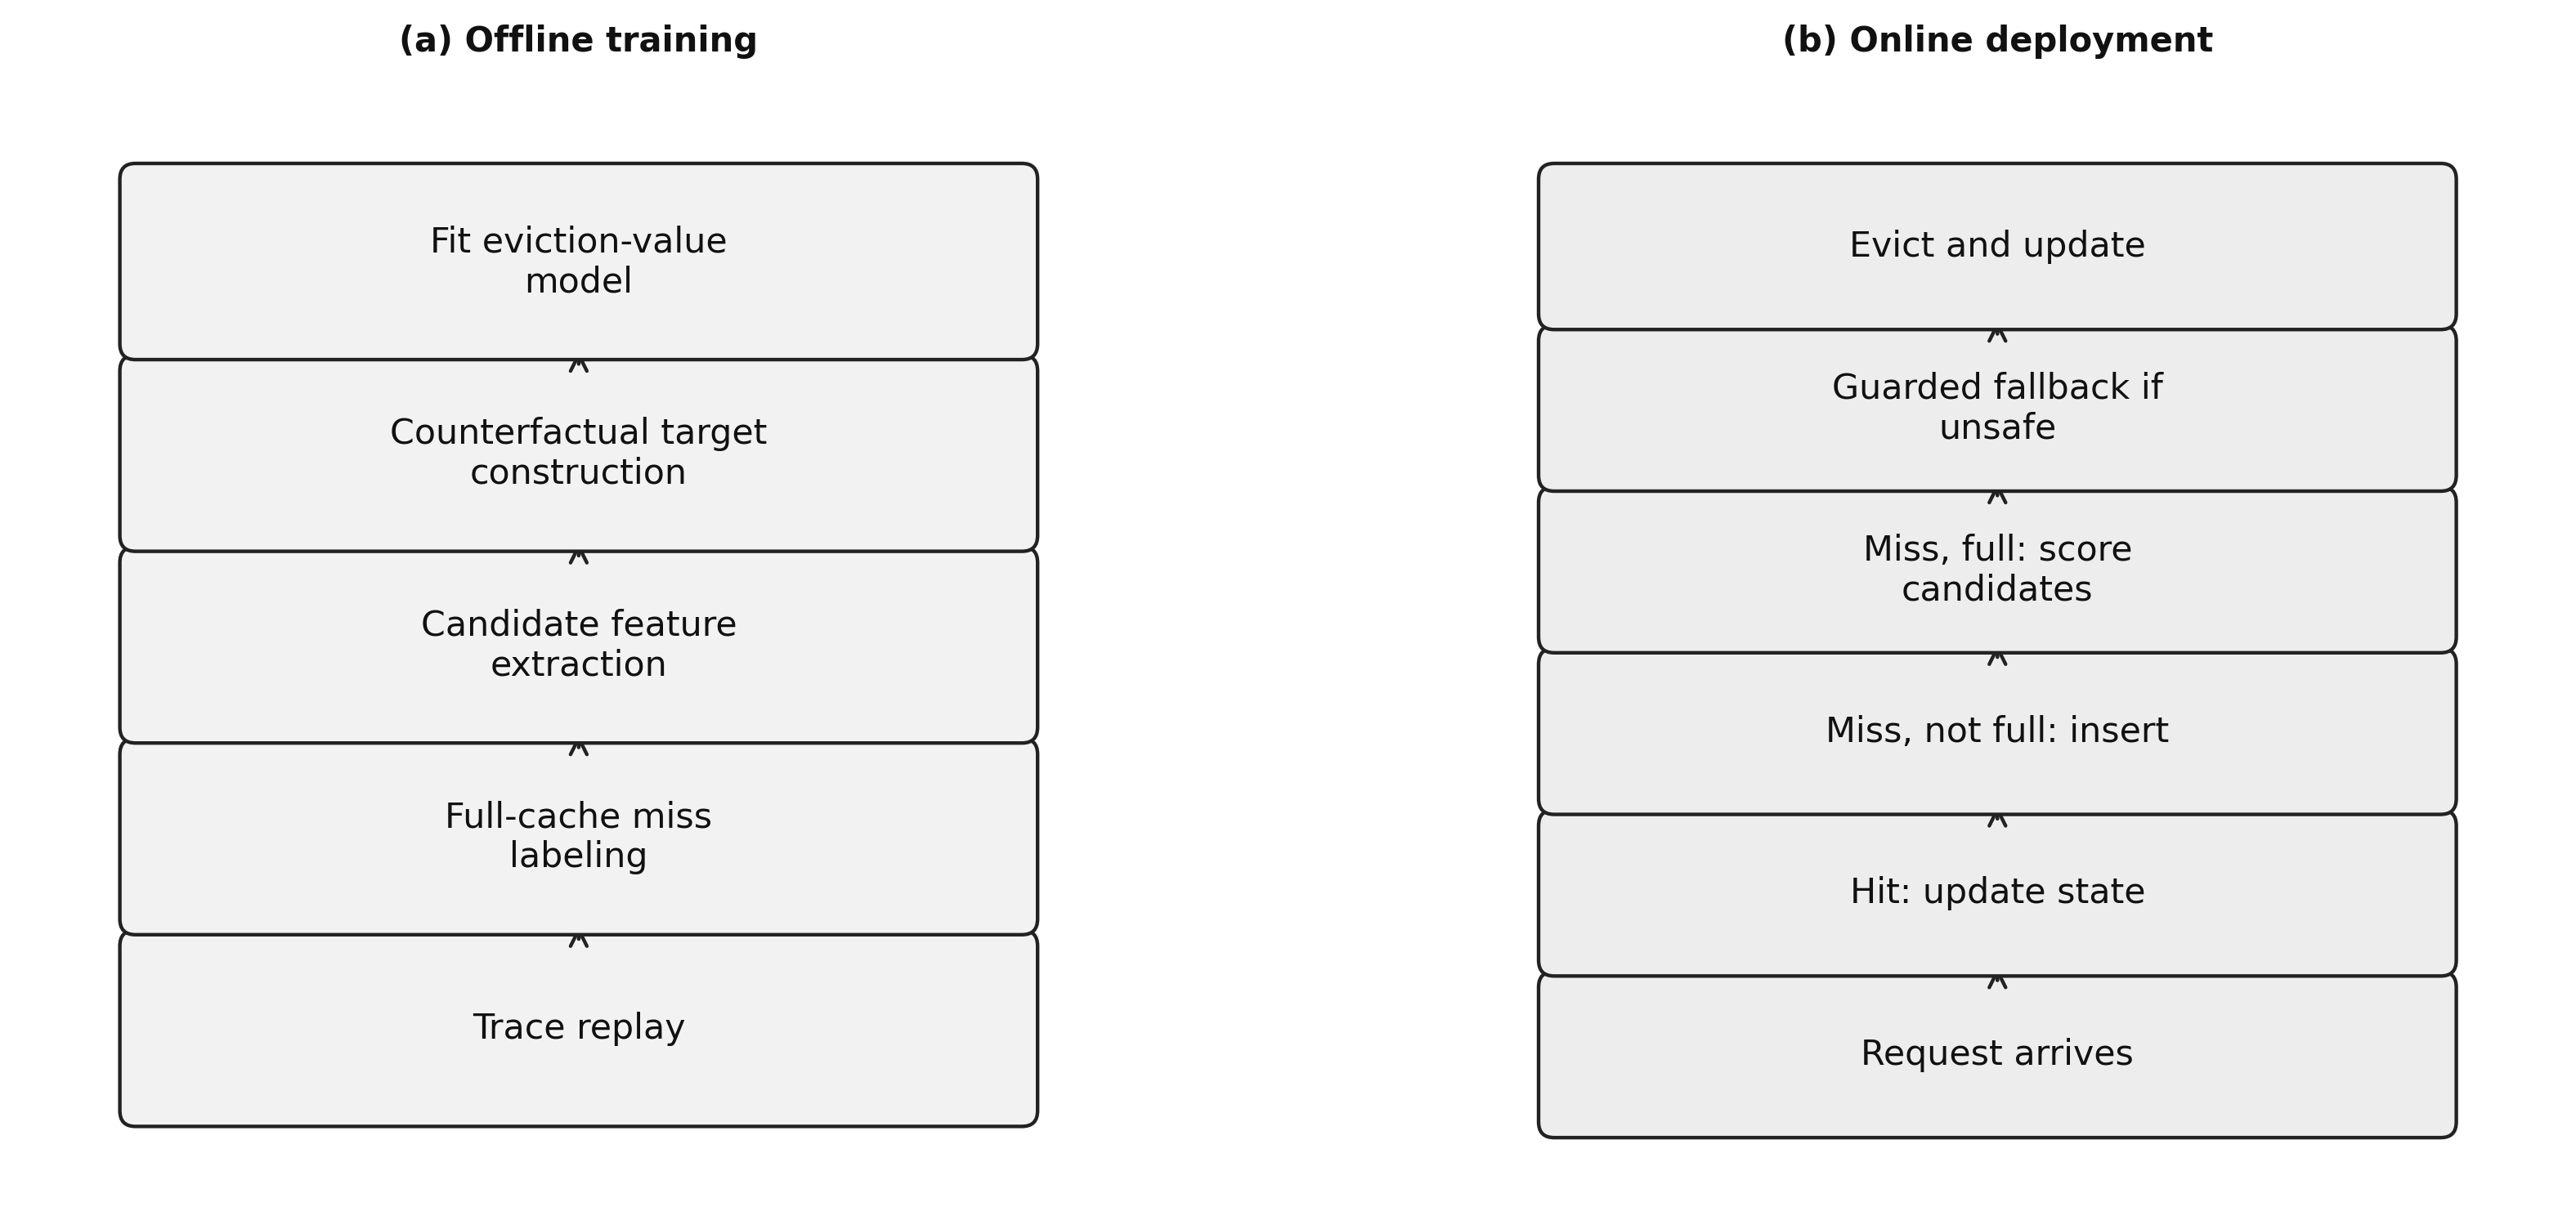
\includegraphics[width=0.96\textwidth]{figures/method_overview.png}
\caption{Conceptual overview of the eviction-value workflow. Offline replay is used to construct candidate-level training examples and finite-horizon loss targets, a supervised scorer is fitted to estimate decision-time eviction loss, and the online policy evicts the candidate with minimum predicted loss. An optional lightweight fallback layer can temporarily delegate control to a conservative baseline when repeated local signals indicate unsafe learned decisions.}
\label{fig:method_overview}
\end{figure*}

In the implementation studied here, candidate-level supervision is generated for the main eviction-value line, a scorer is trained for a chosen replay horizon, and the resulting policy is evaluated in the same simulator used for the reference baselines. The framework records aggregate metrics together with step-level logs so that downstream behavior can be analyzed jointly with fallback activity.

At decision time $t$, the method first builds the candidate feature matrix
\begin{equation}
X_t =
\begin{bmatrix}
x(q_1,t)^{\top}\\
x(q_2,t)^{\top}\\
\vdots\\
x(q_k,t)^{\top}
\end{bmatrix},
\label{eq:candidate_feature_matrix}
\end{equation}
where $\{q_1,\ldots,q_k\}=C_t$ is the current candidate set. The learned scorer then returns the vector of predicted losses
\begin{equation}
\widehat{\ell}_t =
\begin{bmatrix}
\widehat{L}_H(q_1,t)\\
\widehat{L}_H(q_2,t)\\
\vdots\\
\widehat{L}_H(q_k,t)
\end{bmatrix},
\label{eq:predicted_loss_vector}
\end{equation}
and the learned victim is selected by
\begin{equation}
q_t^{*} = \arg\min_{q_i \in C_t} \widehat{L}_H(q_i,t).
\label{eq:workflow_argmin}
\end{equation}
If the optional fallback controller is active, this proposal is passed through the mechanism described in the previous subsection before the final eviction is applied. Learned policies and baselines share the same simulator and trace-loading interface.

\section{Experiments and Discussion}
\label{sec:experiments}


\subsection{Experimental Setup}
\label{subsec:experimental_setup}

The experiments are designed to evaluate the proposed eviction-value framework under a controlled replay protocol. All policies are executed within a common simulator using the same processed traces, cache capacities, request ordering, and trace-loading interface. This unified execution setting is important because it reduces confounding from preprocessing differences, trace-format inconsistencies, and policy-specific replay semantics. Consequently, observed differences in performance can be attributed more directly to differences in eviction behavior.

The empirical focus is the main candidate-scoring policy, \texttt{evict\_value\_v1}, together with a selected set of classical, predictive, and robust reference policies from the learning-augmented caching literature \cite{lykouris2021competitive_caching,antoniadis2020online_metric_untrusted,wei2020better_simpler_lac,chledowski2021robust_lac_experimental}. These baselines are included because they represent the most relevant practical comparison points for online paging under imperfect predictive information. Other policy families implemented in the broader codebase are treated as exploratory or contextual comparisons and are not part of the main empirical claim unless their results are explicitly reported.

The evaluation has two complementary components. The first is \emph{offline scorer construction and selection}. In this component, candidate-level examples are generated from replayed eviction decisions, finite-horizon loss labels are constructed, and model families are compared using target-quality metrics that assess how well the learned scorer approximates the proposed supervision objective. The second is \emph{online replay evaluation}, in which the induced policy is executed in the same simulator as the reference baselines and compared through downstream replay performance. This separation is methodologically important because strong performance on an offline proxy does not necessarily translate into the best online replacement decisions once the scorer is embedded in the full decision loop.

To isolate the eviction-choice problem, the study is conducted in the standard unweighted paging setting with fixed cache capacity and unit miss cost. The principal downstream metric is therefore the total number of cache misses over the replayed request sequence. Claims are restricted to what is directly supported by the reported evaluation outputs below.

\subsection{Datasets, Baselines, and Evaluation Metrics}
\label{subsec:datasets-baselines-metrics}

The empirical study is organized around a common replay interface applied to heterogeneous request traces and a baseline pool chosen to reflect the most relevant practical comparison points for learning-augmented paging. Reported results are restricted to the artifact-backed trace, capacity, and policy subset instantiated by the designated evaluation pipeline.

The baseline pool is selected to cover four comparison roles: classical paging references, CLOCK-family structural references, predictive paging references, and robust learning-augmented controllers. Classical and CLOCK-family references include least-recently used eviction, SIEVE, and FIFO-Reinsertion, which remain essential lightweight anchors for unweighted online caching \cite{belady1966replacement_algorithms,fiat1991competitive_paging,zhang2024sieve}. Predictive and robust references include predictive marker, trust-and-doubt-style control, a regret-driven selective-trust gating controller (REST), and the blind-oracle/LRU combiner \cite{lykouris2021competitive_caching,antoniadis2020online_metric_untrusted,wei2020better_simpler_lac,chledowski2021robust_lac_experimental,im2022parsimonious_lac,rohatgi2020near_optimal_caching}. These methods are used because they represent strong and practically relevant reference points when predictions are informative but imperfect.

Within the learned-policy family, the main method studied in this paper is \texttt{evict\_value\_v1}, which predicts a candidate-specific finite-horizon downstream eviction loss and evicts the candidate with minimum predicted loss. The framework also implements an optional guard that can temporarily defer to a conservative fallback policy when recent online behavior indicates locally unsafe learned decisions; this guard is an implementation safeguard evaluated only as an ablation in the present study, and we do not claim that it improves end-to-end miss ratio unless future experiments support it. Other policy families implemented in the repository, including a standalone marker-style policy, a robust follow-the-prediction combiner with marker fallback, pairwise-ranking variants, sentinel-style guards, and additional exploratory controllers, are retained for contextual analysis and ongoing research development, but they are not treated as central baselines for the present manuscript unless their results are explicitly reported in the canonical artifact bundle.

Table~\ref{tab:trace_families} summarizes the workload families relevant to the present study from a manuscript perspective. The table is intentionally phrased at the family level to separate source provenance from the narrower question of which canonical artifacts are currently reported. Table~\ref{tab:main_policy_families} summarizes the main policy families used in the empirical comparison.

\begin{table}[!htbp]
\centering
\caption{Trace families in the artifact-backed evaluation. The repository supports additional workloads; reported results are restricted to the canonical artifact subset.}
\label{tab:trace_families}
\small
\begin{tabular}{p{2.8cm} p{4.3cm} p{5.0cm}}
\hline
\textbf{Trace family} & \textbf{Representative source} & \textbf{Role in this work} \\
\hline
BrightKite & BrightKite mobility trace \cite{cho2011friendship_mobility} & Public request stream with heterogeneous locality structure for controlled replay evaluation. \\
Citi Bike & Citi Bike system data \cite{citibike_system_data} & Public event stream used to derive replayable request sequences under a common preprocessing interface. \\
SPEC CPU2006 & SPEC CPU2006 benchmark descriptions \cite{henning2006spec_cpu2006} & Classical systems-style trace family providing a contrasting locality regime. \\
Wikimedia pageviews & Wikimedia pageview dumps \cite{wikimedia_pageviews} & Large public page-access source for replay-based cache evaluation. \\
Production-style cache traces & Twitter cache clusters, SHARDS-related resources, and open cache-workload sources \cite{yang2020twitter_cache_clusters,waldspurger2015shards,cachemon_open_source_cache_dataset,cachelib_cachebench_fb_hw_eval} & Manifest-based or documented production-style workloads used to broaden workload diversity in the repository and, when artifact-backed, in the manuscript evaluation. \\
\hline
\end{tabular}
\end{table}

\begin{table}[!htbp]
\centering
\caption{Main policy families in the empirical comparison. A diagnostic-only blind-oracle variant used for internal sanity checks is excluded from the reported comparisons.}
\label{tab:main_policy_families}
\small
\begin{tabular}{p{2.2cm} p{2.3cm} p{6.6cm}}
\hline
\textbf{Label} & \textbf{Category} & \textbf{Role in evaluation} \\
\hline
LRU & Classical baseline & Standard recency-based eviction reference \cite{belady1966replacement_algorithms}. \\
SIEVE & Classical baseline & CLOCK-family turn-key eviction algorithm using a single FIFO queue and an advancing hand pointer over retained objects \cite{zhang2024sieve}. \\
FIFO-Reinsertion & Classical baseline & CLOCK / Second-Chance family baseline that reinserts a retained survivor at the head of the queue rather than advancing a hand \cite{zhang2024sieve}. \\
PredMk & Predictive baseline & Prediction-aware marker-style paging baseline \cite{lykouris2021competitive_caching}. \\
BO/LRU & Combiner baseline & Blind-oracle/LRU practical combiner baseline \cite{wei2020better_simpler_lac}. \\
T\&D & Robust baseline & Trust-and-doubt-style controller for untrusted predictions \cite{antoniadis2020online_metric_untrusted}. \\
REST & Heuristic baseline & Regret-driven selective-trust gating controller that switches between a predictor-driven eviction rule and an LRU fallback based on delayed online feedback. \\
EV & Proposed method & Candidate-level finite-horizon eviction-value predictor. \\
\hline
\end{tabular}
\end{table}

The primary evaluation metric is the total number of cache misses incurred during online replay. We also report hit rate and, where useful for interpretation, miss deltas relative to the LRU baseline. For offline scorer analysis, we additionally use target-quality diagnostics such as regret-style error summaries, Top-1 agreement, and disagreement-oriented statistics. These auxiliary quantities help interpret the learned scorer, but downstream replay performance remains the decisive criterion.

\subsection{Offline Ablation and Model Selection}
\label{subsec:main_results}

We begin with the offline ablation used to select the scorer configuration for \texttt{evict\_value\_v1}. Table~\ref{tab:evict-value-ablation} and Fig.~\ref{fig:evict-value-ablation} summarize validation and test regret across replay horizons and model families. These results are used to characterize the learnability of the candidate-level target and to motivate the scorer configuration carried into the main policy line.

Two patterns are clear. First, the nonlinear tree-based models are consistently stronger than the linear ridge baseline. Across all three replay horizons, ridge incurs substantially larger regret than either \texttt{hist\_gb} or \texttt{random\_forest}. This indicates that the eviction-value target is not well captured by a simple linear approximation and benefits from a more flexible scorer.

Second, shorter replay horizons are stronger in the current artifact set. Horizon $H=4$ gives the best validation regret for \texttt{hist\_gb} and the best test regret for \texttt{random\_forest}, while performance deteriorates as the horizon increases to $8$ and $16$. This trend is consistent with the intended role of the target: a shorter horizon appears to provide a cleaner and more learnable proxy for local eviction harm, whereas longer horizons introduce additional downstream interactions that are harder to model accurately.

The Top-1 results support the same interpretation. On both validation and test splits, the tree-based models achieve lower Top-1 error than ridge across the evaluated horizons, suggesting that nonlinear scorers preserve the candidate ordering needed for eviction decisions more effectively than a linear baseline. At the same time, the gap between \texttt{hist\_gb} and \texttt{random\_forest} is modest relative to their shared advantage over ridge. The main methodological conclusion is therefore about the value of nonlinear scoring and short-horizon supervision, not about one tree-based model being universally dominant.

Taken together, these ablation results support a conservative model-selection conclusion: within the current artifact-backed evidence, the candidate-level eviction-value framework is strongest with a short replay horizon and a nonlinear scorer. This evidence does not by itself establish superiority in end-to-end online replay, but it does show that the proposed target yields a meaningful and learnable signal for downstream eviction scoring.

\begin{table}[!htbp]
\centering
\caption{Offline ablation for \texttt{evict\_value\_v1} across replay horizons and model families. Lower regret is better, and lower Top-1 error is better.}
\label{tab:evict-value-ablation}
\small
\setlength{\tabcolsep}{5pt}
\begin{tabular}{r l r r r r}
\toprule
Horizon & Model & Val.\ regret & Test regret & Val.\ Top-1 & Test Top-1 \\
\midrule
4  & hist\_gb       & 0.0091 & 0.0055 & 0.0174 & 0.0316 \\
4  & random\_forest & 0.0134 & 0.0046 & 0.0154 & 0.0264 \\
4  & ridge          & 0.0649 & 0.0150 & 0.0503 & 0.0832 \\
8  & hist\_gb       & 0.0203 & 0.0104 & 0.0157 & 0.0362 \\
8  & random\_forest & 0.0240 & 0.0120 & 0.0177 & 0.0267 \\
8  & ridge          & 0.0880 & 0.0384 & 0.0377 & 0.0795 \\
16 & hist\_gb       & 0.0394 & 0.0196 & 0.0203 & 0.0365 \\
16 & random\_forest & 0.0431 & 0.0178 & 0.0157 & 0.0249 \\
16 & ridge          & 0.1166 & 0.0850 & 0.0277 & 0.0826 \\
\bottomrule
\end{tabular}
\end{table}

\begin{figure}[!htbp]
    \centering
    
\includegraphics[width=\columnwidth]{figures/figure4_ablation.png}
    \caption{Offline ablation for \texttt{evict\_value\_v1} across replay horizons and model families. The figure summarizes validation and test regret for the configurations shown in Table~\ref{tab:evict-value-ablation}. Lower is better.}
    \label{fig:evict-value-ablation}
\end{figure}

\subsection{End-to-End Online Replay Evaluation Across Available Capacities}
\label{subsec:end_to_end_capacities}

In addition to the offline ablation above, we report end-to-end online replay results for all eight policies in Table~\ref{tab:main_policy_families}, evaluated under the common simulator described in Section~\ref{subsec:experimental_setup} across the seven trace families in Table~\ref{tab:trace_families}, at 50{,}000 requests per trace. At the time of writing, this evaluation has been completed at cache capacities 32, 64, and 128 slots; capacity 256 has not yet been evaluated end-to-end and is not reported in this paper. We are explicit about this boundary because the capacity-128 result discussed below is itself non-monotonic relative to capacities 32 and 64, and we judged it more important to report and analyze the existing three-point trend honestly than to extend further computation into a larger capacity sweep before doing so.

Table~\ref{tab:available-capacities-trend} reports mean replay misses, averaged across the seven trace families, for each policy at each evaluated capacity, and Fig.~\ref{fig:available-capacities-trend} visualizes the same data together with \texttt{evict\_value\_v1}'s relative gap against the three strongest lightweight baselines (LRU, SIEVE, and FIFO-Reinsertion).

\begin{table}[!htbp]
\centering
\caption{End-to-end online replay evaluation: mean misses across the seven trace families in Table~\ref{tab:trace_families} (50{,}000 requests/trace), at each evaluated cache capacity. Capacity 256 has not yet been evaluated end-to-end.}
\label{tab:available-capacities-trend}
\small
\begin{tabular}{l r r r}
\toprule
Policy & Cap.\ 32 & Cap.\ 64 & Cap.\ 128 \\
\midrule
LRU              & 34667.1 & 33650.1 & 32495.6 \\
SIEVE             & 35313.6 & 34362.7 & 33279.3 \\
FIFO-Reinsertion  & 34688.0 & 33672.1 & 32530.6 \\
PredMk            & 34843.9 & 33773.1 & 32664.6 \\
T\&D              & 35087.0 & 33998.7 & 32928.9 \\
BO/LRU            & 34668.6 & 33651.3 & 32496.9 \\
REST              & 34667.1 & 33650.1 & 32495.6 \\
EV (proposed)     & 36344.1 & 34409.0 & 36316.6 \\
\bottomrule
\end{tabular}
\end{table}

\begin{figure}[!htbp]
\centering

\includegraphics[width=\linewidth]{figures/figure_available_capacities_trend.png}
\caption{Capacity-trend comparison across the available evaluated capacities (32, 64, 128; capacity 256 not evaluated in this revision). (a) Mean replay misses per policy at each capacity, averaged across the seven trace families. (b) \texttt{evict\_value\_v1}'s relative miss gap against LRU, SIEVE, and FIFO-Reinsertion at each capacity; positive values indicate more misses than the baseline. The LRU and FIFO-Reinsertion gap curves nearly coincide because the two baselines have nearly identical miss counts in the averaged replay; distinct line styles and markers are used to keep them visually separable. The non-monotonic widening at capacity 128 is discussed in Section~\ref{subsec:discussion_analysis} and Section~\ref{subsec:limitations}.}
\label{fig:available-capacities-trend}
\end{figure}

Three observations follow directly from this available-capacity replay. First, \texttt{evict\_value\_v1} does not improve on LRU, SIEVE, FIFO-Reinsertion, or REST on average at any of the three evaluated capacities: its mean-miss gap relative to LRU is $+4.84\%$ at capacity 32, $+2.26\%$ at capacity 64, and $+11.76\%$ at capacity 128 (equivalently $+2.92\%$, $+0.13\%$, and $+9.13\%$ against SIEVE, and $+4.77\%$, $+2.19\%$, and $+11.64\%$ against FIFO-Reinsertion). REST is numerically tied with LRU at all three evaluated capacities, so the same average gap applies there as well. This is a negative end-to-end result for the proposed policy relative to the strongest baselines in our pool, and we report it directly rather than restricting the paper's empirical claims to the offline ablation evidence above.

Second, the other reference policies cluster tightly around LRU at every evaluated capacity. \texttt{blind\_oracle\_lru\_combiner} (BO/LRU) and \texttt{rest\_v1} (REST) are numerically indistinguishable from LRU ($0.00\%$ gap) at all three capacities, FIFO-Reinsertion stays within $0.11\%$ of LRU throughout, and SIEVE, T\&D, and PredMk remain within roughly $0.4$--$2.4\%$ of LRU at every capacity. \texttt{evict\_value\_v1} is the only policy in the comparison whose gap exceeds $5\%$ at any evaluated capacity, and the only one whose relative position worsens between capacity 64 and capacity 128 rather than tracking the otherwise stable ordering of the other seven policies.

Third, the capacity trend for \texttt{evict\_value\_v1} is non-monotonic: the gap narrows from capacity 32 to capacity 64 and then widens sharply at capacity 128, rather than improving or degrading smoothly with capacity. We examine this pattern at the workload level next, and return to its likely cause in the Discussion and Limitations.

\subsection{Workload-Specific Breakdown}
\label{subsec:workload_breakdown}

Table~\ref{tab:family-capacity-gap} reports \texttt{evict\_value\_v1}'s relative miss gap against LRU separately for each of the seven trace families at each evaluated capacity, rather than only as the family-averaged numbers in Table~\ref{tab:available-capacities-trend}.

\begin{table}[!htbp]
\centering
\caption{\texttt{evict\_value\_v1} relative miss gap against LRU, by trace family and evaluated capacity. Positive values indicate more misses than LRU (worse).}
\label{tab:family-capacity-gap}
\small
\begin{tabular}{l r r r}
\toprule
Trace family & Cap.\ 32 & Cap.\ 64 & Cap.\ 128 \\
\midrule
BrightKite    & $+10.47\%$ & $+10.72\%$ & $+50.91\%$ \\
Citi Bike     & $+7.90\%$  & $+4.70\%$  & $+45.49\%$ \\
CloudPhysics  & $+0.72\%$  & $+1.57\%$  & $+3.10\%$ \\
MetaCDN       & $+22.37\%$ & $+2.73\%$  & $+17.62\%$ \\
MetaKV        & $+1.70\%$  & $+0.01\%$  & $+0.76\%$ \\
Twemcache     & $+1.84\%$  & $+3.16\%$  & $+14.06\%$ \\
Wikimedia$^\dagger$ & $+0.00\%$  & $+0.00\%$  & $+0.00\%$ \\
\bottomrule
\end{tabular}
\\[3pt]
\footnotesize $^\dagger$Degenerate at every evaluated capacity: all eight policies reach 50{,}000/50{,}000 misses (0\% hit rate), because the working set exceeds even the largest evaluated capacity. Not informative for cross-policy comparison.
\end{table}

Two patterns stand out. First, Wikimedia pageviews is degenerate at every evaluated capacity, as noted in the table, and we exclude it from substantive interpretation. CloudPhysics and MetaKV remain close to LRU at every capacity (at most $+3.10\%$ and $+1.70\%$, respectively), consistent with the family-averaged picture in Table~\ref{tab:available-capacities-trend}.

Second, the capacity-128 widening is concentrated in, but not limited to, two families. BrightKite and Citi Bike show the largest gaps at capacity 128 ($+50.91\%$ and $+45.49\%$, respectively), up sharply from roughly $+10\%$ or less at capacities 32 and 64. MetaCDN and Twemcache also show double-digit gaps at capacity 128 ($+17.62\%$ and $+14.06\%$), though their capacity-32/64 trajectories differ from BrightKite's and Citi Bike's: MetaCDN's gap is actually largest at capacity 32 ($+22.37\%$), drops to $+2.73\%$ at capacity 64, and rises again at capacity 128, a U-shaped pattern rather than a monotonic one, while Twemcache's gap increases steadily across all three capacities ($+1.84\%$, $+3.16\%$, $+14.06\%$). In total, four of the six non-degenerate families show a capacity-128 gap above $10\%$, while the remaining two (CloudPhysics, MetaKV) stay below $3.1\%$ throughout. We therefore describe the capacity-128 degradation as broad-based rather than as an artifact specific to two outlier traces, while still noting that BrightKite and Citi Bike are the most extreme cases.

Taken together with the offline ablation in Section~\ref{subsec:main_results}, the capacity-128 degradation documented above is broad-based across workload families rather than an artifact of a single outlier trace, reinforcing rather than qualifying away the negative end-to-end result already reported in Section~\ref{subsec:end_to_end_capacities}. We discuss its likely cause in Section~\ref{subsec:discussion_analysis} and revisit it in Section~\ref{subsec:limitations}.

\subsection{Discussion and Analysis}
\label{subsec:discussion_analysis}

The present results are most informative when interpreted through the central modeling choice of the paper: the proposed method is organized around a decision-aligned supervision target for candidate-level eviction scoring rather than around a global trust-calibration rule. This distinction is important because cache replacement is inherently a local comparative decision. At a full-cache miss, the policy must decide which currently cached item is least harmful to remove, not merely whether predictive information should be trusted in the abstract. From this perspective, the most direct question is not whether the advice appears accurate in isolation, but whether the learned target helps rank the available eviction candidates in a way that improves the actual online choice.

Viewed in this way, the main contribution of the current results is methodological. The offline ablation indicates that replay-based candidate supervision provides a meaningful route for translating predictive context into eviction decisions; tree-based scorers consistently outperform the linear ridge baseline across replay horizons, supporting candidate-level downstream supervision as a viable learning target.

The replay-horizon analysis provides a second useful insight. Within the current artifact set, shorter replay horizons yield the strongest regret values, with $H=4$ performing best among the evaluated settings, consistent with the intended interpretation that longer horizons incorporate harder-to-model downstream interactions.

More broadly, these findings suggest that supervision-target design deserves attention comparable to that given to the predictive signal itself. A candidate-level downstream-loss target remains a proxy, but it is defined directly at the decision point, which gives it a clearer operational interpretation than a trust score or an indirect action surrogate.

At the same time, the interpretation of these results should remain cautious, and the end-to-end evaluation in Section~\ref{subsec:end_to_end_capacities} sharpens rather than removes that caution. The replay-based loss studied here is finite-horizon and local rather than globally optimal, and the offline scorer-selection ablation does not by itself establish superiority in full end-to-end online replay. The explicit end-to-end evidence we now report directly answers that question, and the answer is negative: across all three evaluated capacities, \texttt{evict\_value\_v1} incurs more replay misses than LRU, SIEVE, and FIFO-Reinsertion, with the gap widening sharply and non-monotonically at capacity 128. Likewise, the broader framework includes guarded variants whose end-to-end effect remains unmeasured in the present study (see Limitations). The current results therefore support the proposed supervision target and scoring formulation as a learnable and well-motivated way to pose the eviction-decision problem, but they do not support a claim of downstream competitiveness, robustness across workload regimes, or effective fallback control in deployment; on the contrary, the end-to-end evidence weighs against competitiveness at every capacity evaluated so far.

A natural question is why a learnable, decision-aligned offline target would translate into a policy that underperforms LRU, SIEVE, and FIFO-Reinsertion online, and why the gap would widen specifically at capacity 128 rather than growing smoothly with capacity. We do not have a fully confirmed causal account, but the evidence gathered to date points to a structurally plausible mechanism. The supervision target in Eq.~\eqref{eq:eviction_loss} is constructed under a fixed LRU-style continuation rule: each candidate's training label assumes that, after the scored candidate is evicted, the cache continues to evolve under LRU. The deployed policy, however, recursively makes its own, generally non-LRU eviction choices at every subsequent decision. As a replay episode progresses, the policy's realized trajectory therefore increasingly diverges from the LRU-continuation assumption baked into every training label, a form of compounding distribution shift between the labeling-time counterfactual and the deployment-time trajectory. Because each eviction decision scores every one of the $k$ resident candidates, a larger capacity gives the policy more candidates to rank per decision over the same request budget, which is consistent with, though does not by itself prove, a larger capacity amplifying this compounding effect. We discuss the supporting and limiting evidence for this account, and what would be needed to confirm it, in Section~\ref{subsec:limitations}.

Taken together, the artifact-backed evidence supports a focused but mixed conclusion. Finite-horizon candidate-level eviction-loss prediction is a plausible and methodologically well-motivated direction for learning-augmented caching, and short-horizon nonlinear scorers are the strongest configuration within the offline ablation. At the current stage, this is best interpreted as evidence in favor of the target design and scoring formulation as an object of study, not as a demonstration of practical superiority over strong lightweight baselines: the end-to-end evaluation directly contradicts a superiority claim at every capacity evaluated so far. We therefore characterize \texttt{evict\_value\_v1}, in its present form, as a decision-aligned supervision study rather than as a practically superior online policy, while SIEVE and FIFO-Reinsertion remain strong, low-overhead baselines that the proposed method does not currently outperform. Stronger end-to-end claims and fallback-reliability claims should be reserved for future work that addresses the capacity-128 finding directly.

\subsection{Overhead and Scalability}
\label{subsec:overhead_scalability}

The proposed method has two distinct computational costs: an offline label-construction cost incurred once per dataset, and an online per-decision cost incurred on every full-cache miss during replay or deployment. We report both below, separating measured wall-clock evidence from complexity analysis.

Constructing the finite-horizon eviction-value dataset used in this paper required simulating a fixed continuation policy forward from every eviction decision considered, which is inherently more expensive than constructing a supervision target that can be read directly from the trace (e.g., next-arrival time); this offline construction step took approximately 10.3 hours of wall-clock time and produced 96 GB across 662 shard files. Model training itself is comparatively inexpensive, since it operates on a bounded sample of the constructed dataset rather than on the full label set directly; fitting all evaluated horizon/model-class configurations together took approximately 7--8 minutes.

At each full-cache miss, \texttt{evict\_value\_v1} constructs a feature vector for every one of the $k$ candidates currently resident in the cache and scores each with the trained model, giving $O(k)$ model-inference calls per miss, where $k$ is the cache capacity. This contrasts with the $O(1)$-per-miss classical baselines in our comparison: LRU evicts via a single recency-ordered removal, and the CLOCK-family baselines in our pool, SIEVE and FIFO-Reinsertion, evict via an amortized $O(1)$ hand-scan or reinsertion-scan respectively, with no per-candidate model inference. This is the expected and inherent cost of candidate-level learned scoring relative to structural eviction rules, and it grows with cache capacity rather than remaining constant.

This complexity comparison is verified directly against our own implementations' source code rather than taken solely from the respective baselines' publications. We have since produced a controlled, capacity-isolated wall-clock benchmark: on a 5{,}000-request prefix of the BrightKite trace, measured on the author's local development machine under tmux rather than on the Wulver HPC cluster or under Slurm, the mean wall-clock cost of an \texttt{evict\_value\_v1} eviction decision was 75.0\,ms, 152.1\,ms, and 316.0\,ms at capacities 32, 64, and 128, respectively -- scaling nearly linearly with capacity, consistent with the $O(k)$ candidate-scoring analysis above. Over the same capacities, LRU and FIFO-Reinsertion averaged approximately 0.001\,ms per timed decision, SIEVE ranged from 0.002\,ms to 0.005\,ms, and REST ranged from 0.04\,ms to 0.18\,ms, four to five orders of magnitude faster than \texttt{evict\_value\_v1} throughout. We report this single-trace, single-run measurement as a controlled overhead probe rather than as a claim of representativeness across all seven trace families.

\subsection{Replay Horizon Selection}
\label{subsec:horizon_selection}

The choice of replay horizon $H$ controls a tradeoff in label quality. A short horizon ties the eviction-value label closely to the immediate consequence of the scored decision, while a long horizon allows the label to absorb increasing variance from the continuation policy's own subsequent choices, effects that are downstream consequences of later decisions rather than of the eviction being scored. We observe this tradeoff empirically: validation MAE, RMSE, top-1 eviction match, and mean regret-vs-oracle all degrade monotonically as $H$ increases from 4 to 8 to 16, for every model class evaluated. This pattern holds not only in aggregate but within every individual trace family represented in our validation sample (BrightKite, CloudPhysics, MetaCDN, Twemcache, and Wikimedia pageviews), suggesting that the advantage of shorter horizons in this framework is not specific to any one workload among those evaluated.
We have not yet evaluated whether this pattern extends to the remaining trace families in our full dataset or whether it interacts with cache capacity; we flag both as open questions for future work rather than claim to have resolved them.

\section{Conclusions and Future Research}
\label{sec:conclusion}

\subsection{Summary of Findings}
\label{subsec:summary_findings}

This paper studied learning-augmented caching through a candidate-level view of the eviction decision. Rather than treating prediction primarily as advice to be trusted or ignored at a global level, the paper formulated each full-cache miss as a structured comparison among the items currently in cache and developed a method that predicts the finite-horizon downstream loss associated with evicting each candidate.

The offline ablation shows that the proposed eviction-value target is learnable, that nonlinear scorers are substantially stronger than a linear ridge baseline, and that shorter replay horizons provide the strongest results within the present artifact set. The overall framework also includes a lightweight, optional fallback layer that can defer to a conservative baseline when recent local behavior appears unsafe; Section~\ref{subsec:limitations} discusses why this remains a design extension rather than a validated empirical contribution in the present study.

More broadly, the study suggests that supervision-target design is a central issue in learning-augmented caching: the value of predictive information depends not only on signal quality, but also on whether that signal is translated into a learning objective matched to the online eviction action.

The end-to-end online replay evaluation across capacities 32, 64, and 128 is more cautionary: \texttt{evict\_value\_v1} does not outperform LRU, SIEVE, or FIFO-Reinsertion at any evaluated capacity, with a non-monotonic gap that widens substantially at capacity 128 (Sections~\ref{subsec:end_to_end_capacities} and~\ref{subsec:limitations}). Stronger end-to-end claims, capacity-256 evaluation, and guarded-deployment evidence are left to future work.

\subsection{Implications of the Proposed Approach}
\label{subsec:implications}

The proposed approach has several implications for learning-augmented cache design. The first is methodological: in cache replacement, the supervision target can be as important as the predictive signal itself. The present study suggests that, because the online action is a structured comparison among currently cached candidates, the learning objective should be defined as close as possible to that decision.

A second implication is that robust learning-augmented caching need not be expressed only through global trust calibration or expert switching. In the present implementation, predictive information is incorporated through candidate-level scoring, and the codebase also includes an optional guard-style extension that can be studied separately. That extension is not used to support the quantitative claims in this revision, so the main evidence here concerns the scoring formulation and its end-to-end replay behavior rather than a validated fallback mechanism.

A third implication concerns evaluation methodology. For cache-control methods, it is not enough to assess the quality of an intermediate predictive signal in isolation. What matters is whether the induced eviction decisions improve downstream replay behavior under a controlled simulator, with clear separation between offline target quality and online policy quality.
\subsection{Limitations}
\label{subsec:limitations}

The results of this study should be interpreted in light of several limitations. First, the main method is evaluated in the standard unweighted paging setting with fixed cache capacity and unit miss cost. This setting is well suited to isolating the eviction-choice problem and maintaining comparability with established reference policies, but it does not by itself establish effectiveness for weighted paging, variable object sizes, retrieval costs, byte-oriented objectives, or broader general-caching settings.

Second, the proposed supervision target is intentionally local and finite-horizon. The replay-based loss is designed as a tractable approximation to downstream eviction harm rather than as a globally optimal objective. As a result, the learned scorer is trained to predict a local decision proxy rather than an offline-optimal replacement rule. This design is central to the practicality of the method, but it also limits the strength of any claim about long-range optimality.

Third, the end-to-end online replay evaluation in Section~\ref{subsec:end_to_end_capacities} shows that, at every evaluated capacity (32, 64, and 128), \texttt{evict\_value\_v1} does not improve on LRU, SIEVE, or FIFO-Reinsertion, and that its gap relative to these baselines widens sharply and non-monotonically at capacity 128, in a pattern that is broad-based across four of the six non-degenerate trace families rather than confined to a single outlier. We have not yet isolated the precise causal mechanism behind this capacity-128 finding with a controlled ablation, so the following account should be read as the leading hypothesis rather than a proven explanation. It is consistent with several independent diagnostic checks: the underlying raw outputs are internally consistent and free of duplication or schema drift; the qualitative reversal reproduces deterministically at request counts far smaller than the canonical evaluation, ruling out a large-scale-only artifact; the implementation contains no capacity-specific branching anywhere in the eviction or feature-construction code; and the two most-affected trace families' share of the training data is the smallest among the seven families but is essentially constant across capacities 32, 64, and 128, so a pure training-data-imbalance account would predict a roughly constant relative disadvantage rather than a sudden widening at capacity 128 specifically. The hypothesis we consider most plausible, discussed further in Section~\ref{subsec:discussion_analysis}, is a compounding distribution shift between the single-step LRU-continuation counterfactual used to construct the supervision target in Section~\ref{subsec:eviction_value_framework} and the policy's actual recursive, non-LRU trajectory once deployed, an effect that plausibly grows with the number of candidates scored per decision and therefore with cache capacity. Confirming this account directly would require either a full-scale targeted replay with per-decision trajectory logging or a small retraining ablation under an alternative continuation rule, both of which we leave to future work. Capacity 256 has not yet been evaluated end-to-end pending further analysis of the capacity-128 finding. Given this evidence, we characterize the present contribution accordingly: \texttt{evict\_value\_v1} is best read as a decision-aligned supervision study that demonstrates a learnable, well-motivated candidate-level target, not yet as a practically superior online eviction policy, and SIEVE and FIFO-Reinsertion remain strong, low-overhead baselines that the proposed method does not currently outperform end-to-end.

Fourth, the paper is methodological and empirical rather than theorem-centered. We do not provide a new competitive-ratio guarantee for the learned policy, and the fallback mechanism is introduced as a practical control layer rather than as a formally proved safeguard. The contribution should therefore be interpreted as a decision-aligned learning framework for cache replacement, not as a replacement for the classical worst-case guarantees available in online algorithms.

Fifth, empirical conclusions in learning-augmented caching remain sensitive to workload characteristics, cache capacities, and replay protocol choices. Even with heterogeneous trace families and strong baselines, performance can vary across regimes. The current results should therefore be read as evidence that candidate-level finite-horizon scoring is a promising direction under the evaluated settings, rather than as a claim of universal superiority.

Sixth, this revision is the work of a single author, and the validation reported here cannot substitute for independent replication by additional authors or institutions. To mitigate, but not eliminate, this risk, the revision relies on repository-level audit trails, schema and replay-artifact validation checks, and explicit negative-result reporting in place of multi-author cross-checking.

Finally, the fallback variants introduce additional design choices, including the early-return window, trigger threshold, monitoring interval, fallback duration, and fallback policy. These choices are operationally interpretable and easy to implement, but they remain heuristic parameters rather than theoretically derived constants. Their value may therefore depend substantially on workload regime and deployment conditions.

Taken together, these limitations define the intended scope of the paper. The study makes a focused case for candidate-level finite-horizon eviction-value prediction as a practical and decision-aligned direction for learning-augmented caching, while leaving broader cost models, stronger guarantees, and more extensive regime analysis to future work.

\subsection{Future Research Directions}
\label{subsec:future_research}

Several research directions follow naturally from this study. First, the candidate-centric framework should be extended beyond unweighted paging to weighted and general-caching models with variable object sizes and heterogeneous miss costs. Second, the learning target itself can be strengthened through richer long-range objectives, alternative continuation rules, or ranking-based supervision, provided such formulations improve downstream replay behavior reproducibly. Third, the optional guarded controller remains heuristic; future work should develop validated fallback policies, broader capacity sweeps including capacity 256, and---where possible---partial theoretical guarantees for restricted candidate-scoring or guarded deployment settings.

\section*{Acknowledgements}

The author thanks Professor Ioannis Koutis for his guidance and support throughout this work. The author also acknowledges the use of the Wulver high-performance computing system at the New Jersey Institute of Technology for part of the experimental evaluation.

\section*{Funding}

The author received no specific funding for this work.

\section*{AI Declaration}

During the preparation of this manuscript, the author used ChatGPT for writing assistance and manuscript refinement, and Perplexity AI for literature exploration and background research. During the implementation stage of the project, the author used Cursor, ChatGPT Codex, and GitHub Copilot for coding assistance, and Gemini for limited recommendations, including assistance with auditing repository artifacts and checking internal consistency between the manuscript and the underlying code and results. All AI-assisted text, code, and analysis were independently verified by the author against the repository's artifacts before inclusion, including dedicated schema-validation, replay-artifact, and negative-result audits documented in the repository; AI assistance was not used to introduce any positive result that is not directly supported by these verified artifacts. The author takes full responsibility for the content of the manuscript, the code, and the reported results.

\section*{Data Availability}

The datasets used in this study are cited in the manuscript and were obtained from their respective public or documented sources. The repository associated with this work contains the code used for data preparation, experiment execution, and analysis:
\url{https://github.com/SoroushVahidi/Augmented-caching}.
Access to specific datasets remains subject to the terms, licenses, and availability conditions of the original data providers.

\section*{Code Availability}

The code used to prepare the data, train the models, run the baseline comparisons, and generate the experimental artifacts is available at:
\url{https://github.com/SoroushVahidi/Augmented-caching}

\section*{Declaration of Competing Interest}

The author declares that there is no known competing financial interest or personal relationship that could have appeared to influence the work reported in this paper.

\bibliographystyle{elsarticle-num}
\bibliography{refs}

\end{document}
